\section{Implementierung der Benutzerschnittstelle}\label{sec:frontend}
Die Benutzerschnittstelle der softwaretchnischen Implementierung wird in Form einer Web-Anwendung auf der Basis von SAPUI5 entwickelt, weswegen dieses Framework eingehend erläutert wird.

\paragraph{SAPUI5} SAPUI5 ist ein von SAP entwickeltes Framework zur Entwicklung von Web-Anwendungen gemäß dem HTML5-Standard mit JavaScript, Cascading Style Sheets (CSS) und XML. Es bietet Möglichkeiten, mit wenig Aufwand mobile Anwendungen zu designen.
Anwendungen in SAPUI5 folgen dem MVC-Prinzip (Model-View-Control). Das Model (Modell) ist die Datenstruktur der Anwendung und ist nicht von den Views (Präsentation) abhängig. In den Views werden die Daten des Models dargestellt. Der/Die Controller (Steuerung) sind verantwortlich für die Steuerung der Anwendung, sie können Inhalte der Views verändern, zwischen Views wechseln und das Model manipulieren.
\cite{Goebels.2017}

\subsection{Softwarearchitektur}
Die Softwarearchitektur der Benutzerschnittstelle ergänzt die zuvor dargestellte Softwarearchitektur des Ereignisverarbeitungsdienstes um eine weitere Komponente. In Abbildung \ref{fig:Softwarearchitektur der Benutzerschnittstelle} wird die ergänzte Softwarearchitektur visualisiert.

Die Benutzerschnittstelle als Komponente der Softwarearchitektur kommuniziert hierbei mit SAP S/4HANA Cloud über offene Schnittstellen. Lesende und schreibende Zugriffe auf die Daten von SAP S/4HANA Cloud werden dabei über die Benutzerschnittstelle realisiert. Desweiteren kann die Benutzerschnittstelle Anweisungen des Ereignisverarbeitungsdienstes empfangen und verarbeiten.

\begin{figure}[H]
	\centering 
    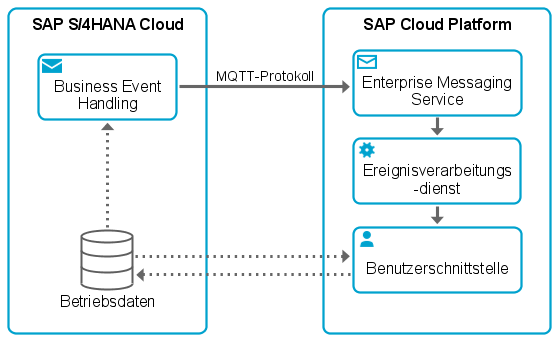
\includegraphics[width=\textwidth]{img/frontntarch.png}	
    \caption[Softwarearchitektur der Benutzerschnittstelle]
    {Softwarearchitektur der Benutzerschnittstelle\protect\footnotemark}
    \label{fig:Softwarearchitektur der Benutzerschnittstelle}
\end{figure}
\footnotetext{Eigene Darstellung}
\footnotetext{Die Abbildung dient lediglich der Visualisierung und ist nicht \ac{BPMN} 2.0 konform.}

\subsection{Benutzung}

\todo{process flows}